\section{Introduction}\label{sec:introduction}

As the High Luminosity LHC~\cite{ZurbanoFernandez:2020cco} (HL-LHC) era approaches, the ATLAS experiment~\cite{PERF-2007-01} has created a HL-LHC focused research and development program~\cite{ATLAS:2020pnm} for software and computing upgrades to address the challenges and opportunities outlined in the ATLAS Software and Computing HL-LHC Roadmap~\cite{CERN-LHCC-2022-005}.
From the 2022 computing model projections, ATLAS does not anticipate being able to store all analysis computations on disk, as even under the ``aggressive'' R\&D scenario, sustained year-on-year budget increases of more than 10\% would be required to meet the disk storage quota required, as seen in~\Cref{fig:atlas-disk-projection}.
To prepare for this reality, ATLAS has begun to explore strategies of trading disk for compute by performing ``on-the-fly'' computations for analysis quantities when possible, rather than reading them from disk.
As part of this approach, ATLAS has been researching the use of columnar analysis --- array programming for data analysis --- for full analysis workflows, given its compute efficient batch data operations and its applications in different software environments and ecosystems.

\begin{figure}
    \centering
    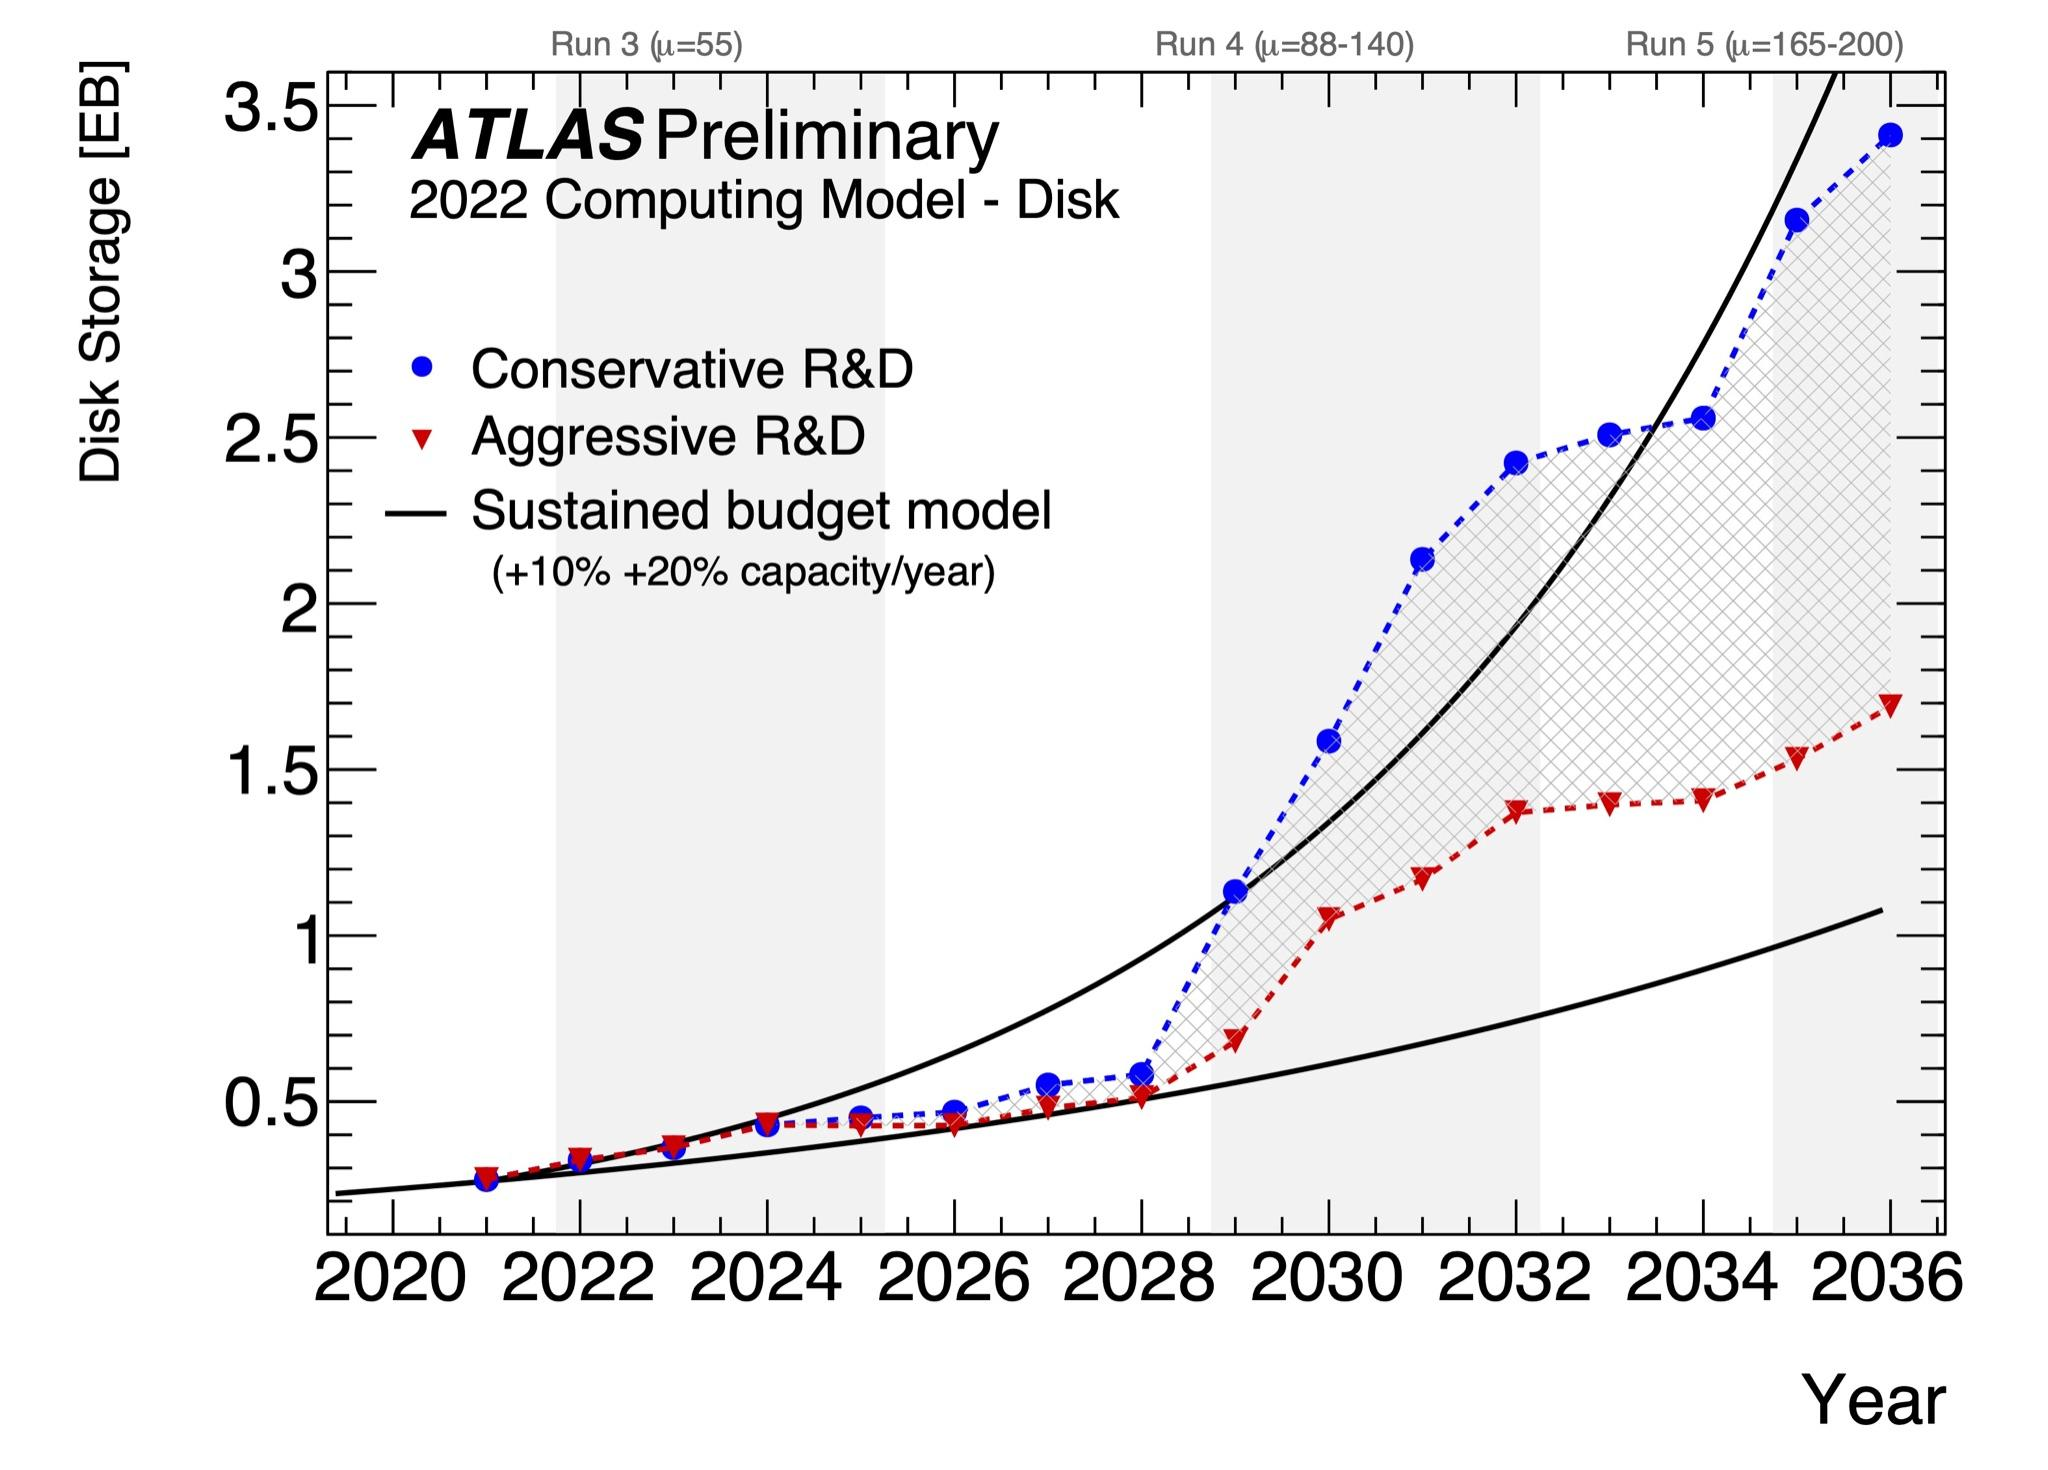
\includegraphics[width=0.7\textwidth]{atlas-disk-projection.png}
    \caption{Projected evolution of disk usage from 2020 until 2036, under the conservative (blue) and aggressive (red) R\&D scenarios.
The grey hatched shading between the red and blue lines illustrates the range of resources consumption if the aggressive scenario is only partially achieved.
The black lines indicate the impact of sustained year-on-year budget increases, and improvements in new hardware, that together amount to a capacity increase of 10\% (lower line) and 20\% (upper line).
The vertical shaded bands indicate periods during which ATLAS will be taking data~\cite{CERN-LHCC-2022-005}.}
    \label{fig:atlas-disk-projection}
\end{figure}
